\chapter{Global observables}
\label{ch:observables}

Circling, gliding and searching for lift combine into the displacement of a whole
flight. We measure its growth, state how effective growth exponents are fitted, and ask
how directional structure varies with take-off region and equipment. The analysis
precedes the phase labels introduced in Chapter~\ref{ch:phases}; Chapter~\ref{ch:models}
then compares these measurements with explicit stochastic-process predictions.

The archive contains \num{\StatMsdParaFlights} paraglider and
\num{\StatMsdHangFlights} hang-glider flights in the retained transport snapshot. A
complete scan of the cleaned archive supplies measurements spanning
\SIrange{10}{10000}{\second}. All retained segments meeting the common-grid cadence and
lag-support requirements enter; there is no cap on the number of flights.
\ifnum\StatSnapshotCurrent=0
The numerical results await regeneration on the archive cleaned with the criteria
of Chapter~\ref{ch:dataset}.
\fi

\begin{table}[htbp]
\centering\small
\caption{Population support in this and the following chapter. The common-grid
analysis includes every eligible flight. The fixed long-flight population supplies
an additional control with identical flights and origins across lags
(Sec.~\ref{sec:quantile-population}).}
\label{tab:chapter3-populations}
\begin{tabular}{@{}lrr@{}}
\toprule
\textbf{Population} & \textbf{Paragliders} & \textbf{Hang gliders}\\
\midrule
Retained cleaned archive & \num{\StatMsdParaFlights} & \num{\StatMsdHangFlights}\\
Eligible on the 10-s grid & \num{\StatRevParaFlights} & \num{\StatRevHangFlights}\\
Fixed long-flight control & \num{\StatRevParaQuantileFixedFlights} & \num{\StatRevHangQuantileFixedFlights}\\
\bottomrule
\end{tabular}
\end{table}

This chapter defines displacement growth for the complete archive, states how effective
exponents are fitted, and measures the directional structure of the retained flights
across regions and equipment groups. Chapter~\ref{ch:global} then removes constant drift
and examines distributional structure, using the same populations.

\FloatBarrier
% TRANSFERRED TO MAIN: original text preserved.
\begingroup\color{red!70!black}
\noindent\textit{Reworked in thesis Section~\ref{sec:fixed-msd}. Original analysis retained below.}\par
\section{Mean-square displacement and growth exponents}
\label{sec:estimator}
\label{sec:obs-global}

Let $\mathbf r_f(t)=(E_f(t),N_f(t))$ be the horizontal position of flight $f$.
Its retained segments form the set $\mathcal S_f$, with $fs$ denoting segment $s$
of flight $f$.

A displacement is
\begin{equation}
  \mathbf X_f(t,\tau)=\mathbf r_f(t+\tau)-\mathbf r_f(t),
  \qquad R_f(t,\tau)=|\mathbf X_f(t,\tau)|.
  \label{eq:displacement-global}
\end{equation}

For segment $fs$, of duration $T_{fs}$, the time-averaged MSD is
\begin{equation}
  \overline{\delta_{fs}^2}(\tau)
    =\frac{1}{T_{fs}-\tau}\int_0^{T_{fs}-\tau}R_f(t,\tau)^2\,\mathrm dt,
  \qquad 0<\tau<T_{fs},
  \label{eq:ta-msd}
\end{equation}
with $t$ measured from the start of that segment.
Only windows lying entirely within a retained segment are admitted, so an increment never
crosses a data gap. Let $n_{fs}(\tau)$ count the admissible windows of segment $fs$ and
$n_f(\tau)=\sum_{s\in\mathcal S_f}n_{fs}(\tau)$ their total over the flight. Combining a
flight's segment sums with those counts gives the flight-level mean
\begin{equation}
  \overline{\delta_f^2}(\tau)
   =\frac{\sum_{s\in\mathcal S_f}n_{fs}(\tau)\,\overline{\delta_{fs}^2}(\tau)}{n_f(\tau)},
  \label{eq:flight-msd}
\end{equation}
a window-count-weighted average of the segment TA-MSDs contributing to that flight.
Averaging further over the population requires a choice of sampling unit:
\begin{equation}
  M_2^{\mathrm{flight}}(\tau)
   =\frac{1}{N_{\mathrm{fl}}(\tau)}\sum_f\overline{\delta_f^2}(\tau),
  \qquad
  M_2^{\mathrm{window}}(\tau)
   =\frac{\sum_f n_f(\tau)\overline{\delta_f^2}(\tau)}{\sum_f n_f(\tau)},
  \label{eq:weights-global}
\end{equation}
where $N_{\mathrm{fl}}(\tau)$ is the number of flights with at least one admissible window.
The first gives each contributing flight equal weight, whereas the second gives each
admissible window equal weight and consequently weights longer flights more strongly.
Substituting Eq.~\eqref{eq:flight-msd} into the second cancels the flight denominators,
\begin{equation}
 M_2^{\mathrm{window}}(\tau)
  =\frac{\sum_f\sum_{s\in\mathcal S_f}n_{fs}(\tau)\overline{\delta_{fs}^2}(\tau)}
        {\sum_f\sum_{s\in\mathcal S_f}n_{fs}(\tau)},
 \label{eq:window-segments}
\end{equation}
so the window average does not depend on how segments are grouped into flights.
Both averages still combine flights made under different meteorological and geographical
conditions.

Figure~\ref{fig:msd} uses a third convention, equal weight per segment:
\begin{equation}
 M_2^{\mathrm{segment}}(\tau)=\frac1{N_{\mathrm{seg}}(\tau)}
 \sum_f\sum_{s\in\mathcal S_f}\overline{\delta_{fs}^2}(\tau),
 \label{eq:segment-msd}
\end{equation}
with $N_{\mathrm{seg}}(\tau)$ the number of segments answering $\tau$.
Only segments with at least eight fixes and support at $\tau$ enter. A split flight
can contribute several segments, and the archive holds
\num{\StatMsdWeightParaSegmentsPerFlight} paraglider and
\num{\StatMsdWeightHangSegmentsPerFlight} hang-glider segments per contributing flight.

In discrete time, a segment $fs$ of $N_{fs}$ fixes
$\mathbf r_0,\ldots,\mathbf r_{N_{fs}-1}$ at interval $\Delta t_{fs}$ contributes
\begin{equation}
 \widehat{\delta_{fs}^2}(k\Delta t_{fs})
 =\frac{1}{N_{fs}-k}\sum_{j=0}^{N_{fs}-k-1}|\mathbf r_{j+k}-\mathbf r_j|^2,
 \qquad 1\le k<N_{fs}.
 \label{eq:discrete-tamsd}
\end{equation}
The common-grid diagnostics below use a \SI{10}{\second} grid, excluding segments with
slower native cadence or fewer than two grid points. Starting times are
$0,\tau,2\tau,\ldots$ within each segment, giving non-overlapping first differences.
Segment sums and origin counts are combined within flights. The duration analysis
in Sec.~\ref{sec:duration-check} instead uses the native-grid segment TA-MSDs,
with its own support and weighting stated there.

The common-grid second moments then receive equal flight weights; baseline quantiles
and higher moments pool windows.

All three averages share one property that limits how far they can be read: the
population contributing to $\tau$ is the set of segments long enough to support it,
so it shrinks as $\tau$ grows. Panel (d) of Fig.~\ref{fig:msd} shows that loss
directly. A slope measured along such a curve combines the growth of displacement
with a change of the flights being averaged, and the two cannot be separated after
the fact. The curves of this section are therefore archive descriptions.
Section~\ref{sec:quantile-population} fixes flights, weights and origins once, and
every exponent and shape comparison in this chapter is taken from that fixed
cohort.

Figure~\ref{fig:msd}a also gives the launch-synchronised average,
$\mathrm{MSD}_{\mathrm{launch}}(t)=\langle|\mathbf r_f(t)-\mathbf r_f(0)|^2\rangle_f$.
Flights occur in different places, seasons and years; this curve describes the
archive without assigning it a common process exponent.

\begin{figure}[htbp]
  \centering
  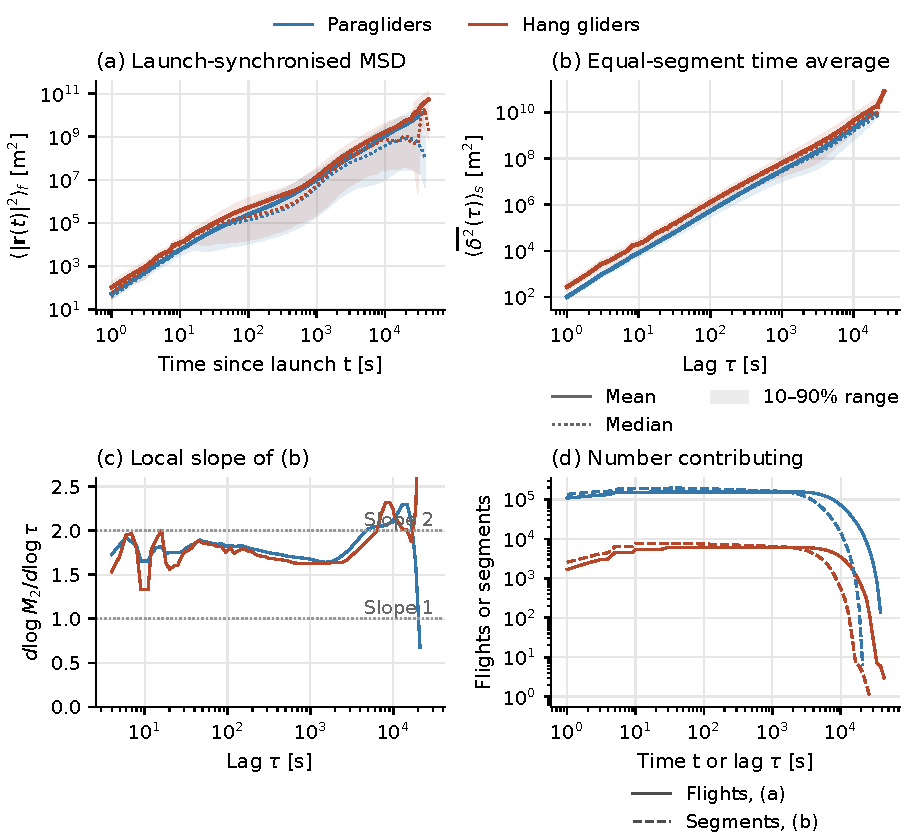
\includegraphics[width=\linewidth]{generated/msd}
  \caption{Archive displacement summaries. (a)~Launch-synchronised average, retained as a
  description of the heterogeneous collection. (b)~Time-averaged MSD, averaged equally
  over retained segments. Solid lines are means, dotted lines medians, and shading the
  10--90\% range across contributing flights in (a), or segments in (b); shading is
  not an uncertainty band on the mean. (c)~Local slope of (b).
  (d)~Contributing flights for (a) and segments for (b), which fall as the lag grows:
  the averaged population changes along every curve in this figure. Panel (a) uses time
  since launch; panels (b,c) use within-segment lag.}
  \label{fig:msd}
\end{figure}

Figure~\ref{fig:msd-weights} evaluates the three conventions on one set of segment
curves, with the same lag support and the same population, so their weights are the only
difference between them. Over
\SIrange{\StatMsdWeightFitMinS}{\StatMsdWeightFitMaxS}{\second} the fitted exponents
span \num{\StatMsdWeightParaAlphaSpread} for paragliders and
\num{\StatMsdWeightHangAlphaSpread} for hang gliders. The amplitudes separate further.
Here $M_2^{\mathrm{window}}$ exceeds $M_2^{\mathrm{segment}}$ at every lag, by up to
\StatMsdWeightParaGapWindowPct\% and \StatMsdWeightHangGapWindowPct\% respectively, with
the largest departure near \SI{3000}{\second}; $M_2^{\mathrm{flight}}$ stays below it by
at most \StatMsdWeightParaGapFlightPct\% and \StatMsdWeightHangGapFlightPct\%. Window
weighting lets the longest flights, which supply most of the admissible origins, set the
level. The equal-flight and equal-segment curves nearly coincide because the archive
averages close to one segment per contributing flight. Departures of this size between
two averages of the same displacement data follow from the weighting convention alone.
They do not establish nonergodicity in a heterogeneous collection.

\begin{figure}[htbp]
  \centering
  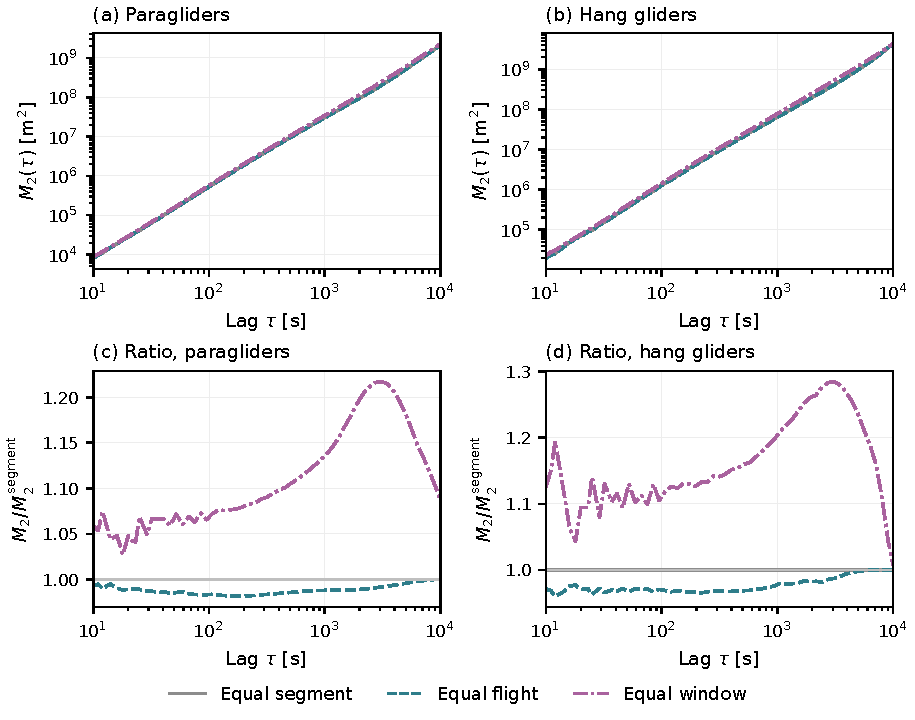
\includegraphics[width=\linewidth]{generated/ch3_msd_weights}
  \caption{The three population weightings of one set of segment TA-MSDs.
  (a,b)~$M_2^{\mathrm{segment}}$ of Eq.~\eqref{eq:segment-msd}, with
  $M_2^{\mathrm{flight}}$ and $M_2^{\mathrm{window}}$ of Eq.~\eqref{eq:weights-global},
  against within-segment lag $\tau$. (c,d)~The same curves divided by
  $M_2^{\mathrm{segment}}$ at the same lag, which is what separates them on these axes.
  All three read the same \num{\StatMsdWeightParaSegments} paraglider and
  \num{\StatMsdWeightHangSegments} hang-glider segment curves, with the lag support of
  Eq.~\eqref{eq:discrete-tamsd}. The comparison isolates the weighting convention; the
  contributing population still changes with lag, identically for all three curves.}
  \label{fig:msd-weights}
\end{figure}

\subsection{Effective and local growth exponents}
\label{sec:exponent}
\label{sec:transport-measure}

The comparison interval is \SIrange{10}{10000}{\second}. For a positive observable
$Y(\tau)$ we distinguish its fitted slope and its local slope,
\begin{equation}
  \log Y(\tau)\simeq a+b\log(\tau/\tau_0),
  \qquad b_{\mathrm{loc}}(\tau)=\frac{\mathrm d\log Y}{\mathrm d\log\tau},
  \label{eq:effective-slope}
\end{equation}
Here logarithms use the stated units, equivalently $\log(Y/Y_0)$, and
$\tau_0=\SI{1}{\second}$. The common-grid and duration reports fit ordinary least
squares in $\log_{10}Y$, with equal weight per admitted lag. A changing local slope
makes $b$ an effective summary of that interval.

Cadence and smoothing can still affect the \SI{10}{\second} end; only long flights
contribute near \SI{10000}{\second}. Coverage and local slopes accompany each fit.
Changing the fitting interval measures sensitivity to curvature and selection.

Sampling uncertainty needs a separate calculation. Windows from one flight, and
flights sharing a site and day, may be dependent. Resampling whole site--day groups
with their complete curves applies the bootstrap~\cite{efron1979} at that level,
assuming exchangeable groups. The baseline curves and slopes below are descriptive;
where intervals are reported, their resampling unit and assumptions are stated.


The drift-removing second difference, and the route geometry that no drift removal can
cancel, enter with the preliminary transport measurements of Chapter~\ref{ch:global}.
The rest of this chapter stays with displacement itself and asks how its direction
depends on where a flight starts and what it flies.

\FloatBarrier
\FloatBarrier
\endgroup

\section{Directional structure, terrain and equipment}
\label{sec:transport-axisroutes}
\label{sec:transport-anisotropy}
\label{sec:transport-environment}

We next ask how directional structure varies across take-off regions and equipment
groups, and which environmental interpretations these contrasts can support.
The quantities differ from the fixed-population collapse test of
Chapter~\ref{ch:global}: launch-time
second moments describe mean motion and spread together, whereas regional
increment covariances describe centred spread over a lag. Their clocks, weighting
and contributing flights must therefore be specified before comparing them.

\subsection{East--north balance in the retained archive}

Isotropy requires the joint displacement law to remain unchanged under rotation.
Equality of east and north second moments is one necessary condition. For positions
measured from launch, define
\begin{equation}
  \rho_{EN}(t)=\frac{\langle E_f(t)^2\rangle_f}{\langle N_f(t)^2\rangle_f},
  \qquad
  \langle E_f(t)^2\rangle_f
  =\operatorname{Var}_f[E_f(t)]+\langle E_f(t)\rangle_f^2.
  \label{eq:archive-directional-ratio}
\end{equation}
This uncentred ratio combines mean motion and spread. Here $t$ is time since
launch, and its contributing flights change with $t$. Unity checks one moment
condition for isotropy.

\begin{figure}[htbp]
  \centering
  \IfFileExists{generated/prelim_isotropy.pdf}{%
    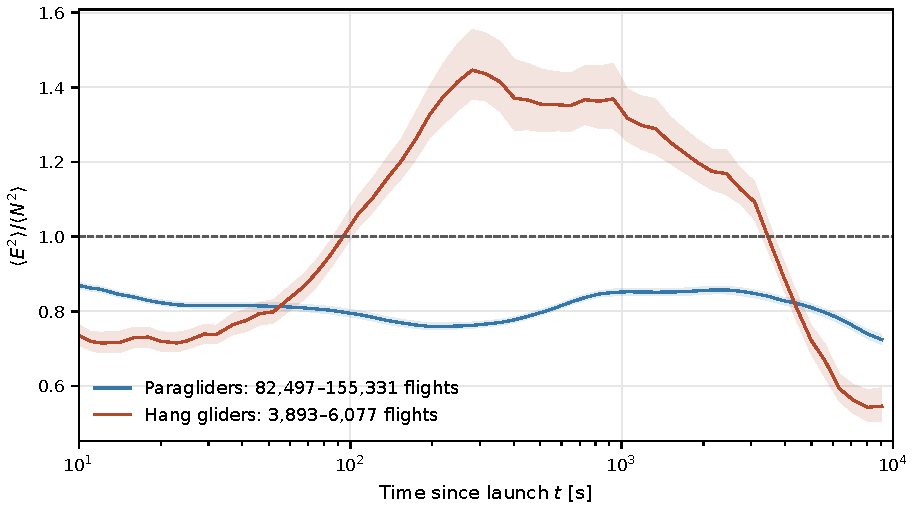
\includegraphics[width=\linewidth]{generated/prelim_isotropy}%
  }{%
    \fbox{\parbox{0.8\linewidth}{\centering\small Figure generated locally by
    \texttt{scripts/reporting/ch2\_dataset/generate\_prelim\_figure.py} from the processed
    dataset on the SSD (not versioned).}}%
  }
  \caption{Archive east--north second-moment ratio against elapsed time since launch.
  Curves show the observed ratio; shading gives the pointwise 10--90\% range from
  \StatPrelimIsoBootResamples\ bootstrap resamples of whole take-off-site-and-day
  groups. Only times with at least \StatPrelimIsoMinFlights\ paired flights and
  \StatPrelimIsoMinClusters\ contributing clusters are shown; legend counts give the
  minimum and maximum flight support along each curve. These are display minima, not
  a precision criterion. Unity is a necessary
  condition for isotropy, not sufficient evidence of it; these bands are not a
  simultaneous confidence statement across all times.}
  \label{fig:prelim-isotropy}
\end{figure}

Over \SIrange{10}{10000}{\second}, the unresampled
ratio ranges from \StatPrelimParaIsoRatioMin\ to \StatPrelimParaIsoRatioMax\ for
paragliders and from \StatPrelimHangIsoRatioMin\ to \StatPrelimHangIsoRatioMax\ for
hang gliders. These are curve extrema, not bootstrap-band limits. The directional
imbalance supports treating east, north and radial displacement separately. It
describes the heterogeneous retained archive; it does not identify whether route
choice, terrain or wind produces the imbalance. The centred regional analysis below
asks how much directional structure remains after subtracting each subgroup's mean.
Launch-referenced positions can retain reacquisition offsets across missing
intervals; within-segment increments avoid bridging those intervals but do not
independently validate their endpoints.

\subsection{Regional principal axes}

For a region $g$, define the centred displacement covariance
\begin{equation}
  \boldsymbol\mu_g(\tau)=\mathbb E[\mathbf X\mid g],\qquad
  \Sigma_g(\tau)=\mathbb E[(\mathbf X-\boldsymbol\mu_g)
                         (\mathbf X-\boldsymbol\mu_g)^\top\mid g]
          =U_g\,\mathrm{diag}(\lambda_1,\lambda_2)\,U_g^\top,
  \label{eq:pca-global}
\end{equation}
with $\lambda_1\ge\lambda_2$. The ratio and whitening below require
$\lambda_2>0$. The leading eigenvector describes the direction of greatest
spread, modulo $180^\circ$; it is an axis, not a signed wind direction. The ratio
$\lambda_1/\lambda_2$ measures anisotropy of the covariance. An axis becomes poorly
determined when the eigenvalues are close. Covariances pool all supported
baseline increment origins within each take-off box, so flights with more
origins receive more weight. They use the eligible regional archive, independently
of the fixed long-flight cohort. The four lags are exactly 10, 100, 1000 and
10000~s, evaluated directly on the 10-s coordinate grid. Increment origins are
spaced by the lag within each segment; no increment crosses a segment boundary.
Each lag uses every flight with supported increments, so the contributing
population can shrink as the lag increases. At least eight flights are required; this
display condition supplies neither an uncertainty interval nor a precision guarantee.

\begin{figure}[htbp]
  \centering
  
\includegraphics[width=\linewidth]{generated/ch3_pca}
  \caption{Regional principal-axis diagnostics in the paraglider eligible archive. Covariances are
  centred before diagonalisation. The principal direction is an axis modulo
  $180^\circ$ and its interpretation depends on the separation of the two eigenvalues.
  Region counts and lag dependence delimit the evidence. These measurements describe
  displacement geometry and do not identify wind. Ellipses and matching coloured
  markers show all four lags: 10, 100, 1000 and 10000~s. Ellipses are normalised
  by the square root of the covariance trace, removing amplitude differences.
  Legends give contributing-flight counts at each lag; angle labels accompany
  the eigenvalue ratios. Changes across lags can also reflect changes in this population.}
  \label{fig:regional-pca}
\end{figure}

\noindent\begin{minipage}{\linewidth}
At \SI{\StatRevParaPcaReferenceLagS}{\second}, the regional comparison is
\begin{center}
\begin{tabular}{@{}lrrr@{}}
\toprule
\textbf{Region} & \textbf{Flights} & $\boldsymbol{\lambda_1/\lambda_2}$ & \textbf{Axis from east} \\
\midrule
Alps & \num{\StatRevParaPcaAlpsFlights} & \StatRevParaPcaAlpsRatio & \SI{\StatRevParaPcaAlpsAngle}{\degree} \\
Pyrenees & \num{\StatRevParaPcaPyreneesFlights} & \StatRevParaPcaPyreneesRatio & \SI{\StatRevParaPcaPyreneesAngle}{\degree} \\
Channel coast & \num{\StatRevParaPcaChannelCoastFlights} & \StatRevParaPcaChannelCoastRatio & \SI{\StatRevParaPcaChannelCoastAngle}{\degree} \\
\bottomrule
\end{tabular}
\end{center}
\end{minipage}\par\medskip
Angles run counterclockwise from east. The Pyrenean axis lies closer to
east--west; its eigenvalue ratio increases towards long lags as support falls,
leaving both route geometry and selection as possible contributors. The coastal
comparison also has unequal principal variances, with thousands of flights at
the reference lag. Its geographical label does not provide an isotropic control.

\paragraph{Environmental constraints across displacement scales.}
In all three regions, the observed ratio $A_g(\tau)=\lambda_1(\tau)/\lambda_2(\tau)$
increases between each pair of successive measured lags. The centred displacement
cloud therefore becomes more elongated as the observation interval lengthens.
This suggests that terrain-guided routes and persistent wind effects become more
visible in displacement geometry when an increment spans enough time to explore
their spatial scale or accumulate their directional contribution. Here $\tau$ is
the duration of an increment starting anywhere inside a supported segment; it is
not the time elapsed since take-off. The four estimates establish an ordering on
the sampled grid, rather than a positive derivative at every intermediate lag.
Where the eigenvalues are differentiable and positive,
\begin{equation}
 \frac{d\log A_g}{d\tau}
 =\frac{\lambda_1'}{\lambda_1}-\frac{\lambda_2'}{\lambda_2}.
 \label{eq:pca-relative-growth}
\end{equation}
An increasing ratio measures faster proportional growth along the principal axis;
both variances may still increase. It does not measure the strength of a force.

\paragraph{Time needed to explore terrain constraints.}
A short increment may sample only a small part of a valley, ridge or accessible
flight corridor. Over a longer interval, the pilot may approach terrain or leave
usable lift and have to turn, follow the valley or remain near the ridge. The
transverse displacement can then grow more slowly than displacement along the
route. This gives a concrete interpretation to the idea of taking time to
``feel the boundary'': the increment must span enough of the route for its
geometry to restrict the observed displacement. In an idealised corridor of
width $L$, transverse displacement is bounded by the corridor width while
longitudinal displacement can continue to grow. A crossing-time estimate is
$L/v_\perp$ for approximately persistent transverse motion, or of order
$L^2/D_\perp$ for diffusive transverse exploration. These are dimensional
examples, not fitted time scales for the flights. Actual mountains are neither
reflecting walls nor impermeable boundaries at every altitude. Pilots may
anticipate a turn, and terrain-linked lift can influence headings immediately.
The ratios already exceed one at 10~s, so the observation does not imply that
orography is irrelevant at short lags.

\FloatBarrier
\paragraph{Wind coherence and accumulated displacement.}
The horizontal wind contribution along a flight is
$\Delta\mathbf r_w(t,\tau)=\int_0^\tau\mathbf w_h(t+s)\,ds$.
A persistent component accumulates with a consistent sign; rapidly changing
components can partly cancel. The covariance of this contribution is
\begin{equation}
 \Sigma_w(t,\tau)=\int_0^\tau\!\int_0^\tau
 \operatorname{Cov}[\mathbf w_h(t+s),\mathbf w_h(t+u)]\,ds\,du.
 \label{eq:wind-integrated-covariance}
\end{equation}
For a stationary scalar component with autocovariance $C_w(s)$, this reduces to
$2\int_0^\tau(\tau-s)C_w(s)\,ds$, the velocity-correlation relation underlying
Taylor's dispersion formula~\cite{taylor1922}. Over an interval shorter than its coherence
time, nearly constant random wind gives a contribution proportional to $\tau^2$;
well beyond an integrable correlation time, the leading growth is generally
linear in $\tau$ when the integrated autocovariance is nonzero. Waiting longer
does not itself make wind more coherent. A weak persistent contribution can
nevertheless become visible after accumulating enough displacement relative to
other sources of spread.

For the centred PCA, a constant wind vector shared by every observation only
adds $\tau\mathbf w_h$ to the mean and disappears on centring. The proposed wind
mechanism must therefore involve variability between flights or increment
origins, temporal or spatial changes of wind, or a response of the chosen route.
As an illustrative calculation, let the background displacement have covariance
$2D\tau I_2$ and let an independent wind component $W$ act along a fixed unit
axis $\mathbf e$. Suppose $W$ varies across the ensemble with variance
$\sigma_w^2$ but remains constant within an increment. Then
\begin{equation}
 \Sigma(\tau)=2D\tau I_2+\sigma_w^2\tau^2\mathbf e\mathbf e^\top,
 \qquad
 \frac{\lambda_1}{\lambda_2}=1+\frac{\sigma_w^2\tau}{2D}.
 \label{eq:wind-anisotropy-example}
\end{equation}
In this example a small $\sigma_w$ delays the scale at which the directional
contribution competes with the background, of order $2D/\sigma_w^2$. The wind
must remain coherent over that scale for this argument to apply. Neither the
diffusive background nor the independent wind model has been fitted here.
In the flights, air-relative motion and wind can be correlated, adding cross
covariances to Eq.~\eqref{eq:wind-integrated-covariance}; a broadly isotropic
distribution of persistent wind directions would also fail to select a common
axis. Thus the growing ratio supports an interpretation in terms of accumulated
environmental guidance, while its attribution requires fixed flight/origin
support, terrain scales along the routes and wind matched to flight time and
altitude. Changing route mixtures and the declining long-lag population can
also contribute to the observed growth.

\paragraph{Rotation, whitening and second-order isotropy.}
Rotation into the principal frame gives uncorrelated components at the lag at which the
covariance was fitted. It does not establish independence or remove temporal
correlations. It cannot improve radial collapse because
\begin{equation}
  |U_g^\top\mathbf X|=|\mathbf X|.
  \label{eq:pca-radius}
\end{equation}
Whitening with the reference covariance,
$\mathbf Z(\tau)=\Sigma_g(\tau_0)^{-1/2}[\mathbf X(\tau)-\boldsymbol\mu_g(\tau)]$,
changes lengths. It sets the covariance to the identity at the reference lag $\tau_0$; it need not
do so at other lags, and it does not imply a rotationally invariant distribution.
If instead each lag has its own positive-definite covariance, then
\begin{equation}
 \mathbf Z_\tau=\Sigma_g(\tau)^{-1/2}
 [\mathbf X_\tau-\boldsymbol\mu_g(\tau)],\qquad
 \operatorname{Cov}(\mathbf Z_\tau)=I_2
 \label{eq:lagwise-whitening}
\end{equation}
by the defining identity of whitening~\cite{kessy2018}. This does enforce
second-order isotropy of each centred increment distribution separately: all
unit-vector projections have variance one and the covariance ellipse is a
circle. With estimated covariances, the equality holds on the same weighted
sample used to fit the transformation; it is not guaranteed on new flights.
Higher-order angular structure can remain, and the resulting normalisation
does not test a common scaling law.

Second-order isotropy of an entire centred vector process would also require
its two-time covariance $K(s,t)=\operatorname{Cov}[\mathbf Y(s),\mathbf Y(t)]$
to satisfy $QK(s,t)Q^\top=K(s,t)$ for every spatial rotation $Q$ and every pair
of times. Equal one-time covariances do not ensure this. For example, two
independent stationary components with unit variance and autocorrelations
$\exp(-a|h|)$ and $\exp(-b|h|)$, with $a,b>0$ and $a\ne b$, have covariance $I_2$ at every
time but different directional memory. Their two-time covariance is diagonal
with unequal entries at nonzero separation, so a quarter-turn changes it.
Moreover, applying a different matrix to each increment lag generally breaks
the additivity needed to interpret those vectors as increments of a single
transformed trajectory. A control that tests whether one spatial transformation
and one scalar scale factor suffice instead fits the transformation at a fixed
reference lag and evaluates covariance shape, angular distributions and
two-time dependence on other scales and flights.

\FloatBarrier
\subsubsection{Independent terrain orientation}
\label{sec:independent-terrain-axis}

An independent geographical reference helps distinguish an observed displacement
axis from an assumed mountain direction. NOAA's ETOPO 2022 elevation model
\cite{noaa_etopo2022} supplies this reference within the same Alpine and Pyrenean
take-off boxes. The construction can be pictured as making a binary map of the
high terrain and fitting an ellipse to the selected map cells: the ellipse's
long axis is the indicative direction of the mountain area.

\paragraph{Construction.}
The numerical recipe is:
\begin{enumerate}[leftmargin=*,itemsep=0.25em,topsep=0.4em]
 \item Crop the ETOPO elevation map to the same Alpine or Pyrenean box used to
 classify flight take-offs.
 \item Retain every fourth cell in longitude and latitude. Starting from the
 15-arc-second ETOPO grid gives one-arc-minute spacing and approximately one
 sixteenth of the original number of cells.
 \item Select the retained cells with elevation $h_i\ge\SI{1000}{\metre}$.
 This produces a binary highland footprint: elevation above the threshold gives
 no additional weight.
 \item Convert the centre of every selected cell from longitude--latitude to
 local WGS84 coordinates $\mathbf q_i=(E_i,N_i)$, in metres from the centre of
 the regional box. Use zero projection height because only the plan-view
 orientation is required.
 \item Assign the area weight $w_i=\cos\varphi_i$, where $\varphi_i$ is the cell
 latitude, to compensate approximately for the decreasing physical width of a
 longitude--latitude cell away from the equator.
 \item Compute the weighted centre and the $2\times2$ spatial covariance of the
 selected cell centres.
 \item Diagonalise that covariance. The eigenvector with the larger eigenvalue
 is the long axis of the footprint; report its angle counterclockwise from east,
 modulo $180^\circ$.
\end{enumerate}
In step 6 the quantities are
\begin{equation}
 \overline{\mathbf q}=
 \frac{\sum_iw_i\mathbf q_i}{\sum_iw_i},\qquad
 C_{\mathrm{terrain}}=
 \frac{\sum_iw_i(\mathbf q_i-\overline{\mathbf q})
                    (\mathbf q_i-\overline{\mathbf q})^\top}
      {\sum_iw_i}.
 \label{eq:terrain-footprint-covariance}
\end{equation}
The eigenvector of $C_{\mathrm{terrain}}$ with the larger eigenvalue is the
long axis of the area-weighted cell cloud.

\paragraph{Interpretation.}
No flight coordinate enters this calculation, and neither the threshold nor the
axis is fitted to the flight PCA. The method estimates the mean elongation of all
terrain above the chosen threshold inside the box. It does not trace a crest,
identify individual valleys or weight the terrain actually crossed by a flight.
The box boundary, plateaux and the curvature of a mountain chain can therefore
affect the result. Repeating the construction at 500 and \SI{1500}{\metre}
measures sensitivity to the operational footprint definition.

\begin{figure}[htbp]
  \centering
  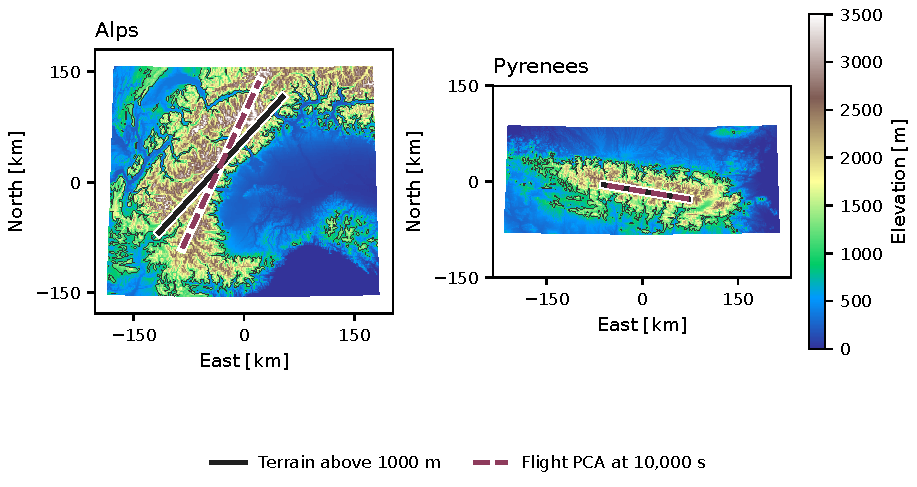
\includegraphics[width=\linewidth]{generated/ch3_terrain_axes}
  \caption{Independent terrain orientation compared with the paraglider
  displacement covariance at \SI{10000}{\second}. Elevation and the
  \SI{1000}{\metre} contour come from ETOPO 2022 \cite{noaa_etopo2022}.
  The solid dark line is the highland-footprint axis; the dashed coloured line
  is the flight PCA axis, translated to the same centre for comparison.
  Line lengths carry no displacement or ridge-length information. Map coordinates
  are kilometres east and north of each box centre.}
  \label{fig:independent-terrain-axes}
\end{figure}

\noindent\begin{minipage}{\linewidth}
The angles, counterclockwise from east and modulo $180^\circ$, are
\begin{center}
\begin{tabular}{@{}lrrr@{}}
\toprule
\textbf{Region} & \textbf{Terrain axis} & \textbf{Flight axis} & \textbf{Separation}\\
\midrule
Alps & \SI{\StatTerrainAlpsAngle}{\degree} & \SI{\StatTerrainAlpsFlightAngle}{\degree} & \SI{\StatTerrainAlpsDifference}{\degree}\\
Pyrenees & \SI{\StatTerrainPyreneesAngle}{\degree} & \SI{\StatTerrainPyreneesFlightAngle}{\degree} & \SI{\StatTerrainPyreneesDifference}{\degree}\\
\bottomrule
\end{tabular}
\end{center}
\end{minipage}\par\medskip
Using thresholds of 500, 1000 and \SI{1500}{\metre} places the terrain axis in
\SIrange{\StatTerrainAlpsMinAngle}{\StatTerrainAlpsMaxAngle}{\degree} in the Alps
and \SIrange{\StatTerrainPyreneesMinAngle}{\StatTerrainPyreneesMaxAngle}{\degree}
in the Pyrenees. These spans describe sensitivity to the footprint definition;
they are not confidence intervals. Decimal values identify the calculation,
not the precision of a physical mountain direction.

The Pyrenean long-lag spread is closely aligned with the independent highland
axis. This supports a geographical association between route orientation and
the range. In the Alps, both axes occupy the northeast--southwest sector, but
the flight axis is about $18^\circ$ more northward than the mean highland axis;
simple parallel alignment is a poorer description there. The curved Alpine
chain and its truncation by the box can contribute to this difference.
Neither comparison identifies a causal terrain effect: wind, route choice and
the long-flight population can also contribute. The PCA uses
\num{\StatTerrainAlpsFlights} Alpine and \num{\StatTerrainPyreneesFlights}
Pyrenean flights at this lag. Their increments can extend beyond the
take-off box, and their tangent frames differ from the single regional terrain
frame. This is an indicative regional comparison, not a measure of terrain
exposure along individual tracks or a test of pilot skill.

\subsubsection{An independent coastal wind reference}
\label{sec:independent-coastal-wind}

For the Channel Coast, an independent wind climatology provides the corresponding
orientation reference. ERA5 hourly reanalysis \cite{era5_hourly}, retrieved through
the Open-Meteo Historical Weather API \cite{open_meteo_historical}, supplies wind
speed and direction at 10 and \SI{100}{\metre} above ground. The reference covers
ten complete years, 2016--2025. It uses nine representative cells: the nearest
ERA5 cells to the centres of a regular $3\times3$ partition of the existing
Channel Coast box. Model selection is explicitly ERA5, on its $0.25^\circ$ grid,
with neither a land-cell preference nor elevation downscaling. This sparse
regional sample is adequate for an indicative orientation comparison; it does
not resolve local coastal lift or reproduce weather along individual flights.

If $s$ is wind speed and $\phi$ the meteorological direction, measured clockwise
from north and indicating where the wind comes from, the east and north
components of air motion are
\begin{equation}
 u=-s\sin\phi,\qquad v=-s\cos\phi,\qquad
 \theta_w=\operatorname{atan2}(\langle v\rangle,\langle u\rangle).
 \label{eq:regional-wind-axis}
\end{equation}
The averages include every archived hour and weight cells by
$\cos(\mathrm{latitude})$ to approximate represented area. Direction angles
are never averaged arithmetically. The resulting \emph{towards} angle is
counterclockwise from east, then reduced modulo $180^\circ$ for comparison
with the undirected PCA axis. Thus a meteorological wind \emph{from}
\SI{\StatWindSurfaceFrom}{\degree} corresponds to the reference axis
\SI{\StatWindSurfaceAngle}{\degree} used here.

\begin{figure}[htbp]
 \centering
 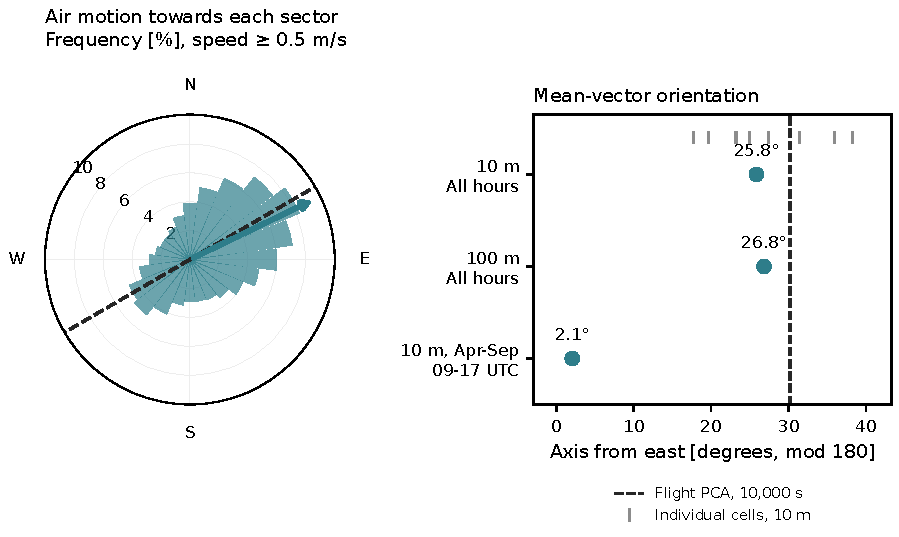
\includegraphics[width=\linewidth]{generated/ch3_channel_wind}
 \caption{ERA5 coastal wind reference and the paraglider covariance axis at
 \SI{10000}{\second}. Left: weighted frequency of air motion \emph{towards}
 15-degree sectors at \SI{10}{\metre}, excluding speeds below
 \SI{0.5}{\metre\per\second} and normalising the retained observations.
 The coloured arrow is the mean wind vector direction, calculated using all
 hours; the dashed line is the undirected flight axis. Right: mean-vector
 axes for the annual \SI{10}{\metre} reference, an annual \SI{100}{\metre}
 check, and a \SI{10}{\metre} April--September, 09--17 UTC check.
 Grey marks show the nine separate annual cell means, not confidence limits.
 The same \num{\StatWindFlights} coastal flights define the PCA reference
 in all three comparisons.}
 \label{fig:independent-coastal-wind}
\end{figure}

The annual surface-wind axis, \SI{\StatWindSurfaceAngle}{\degree}, is close to
the flight axis, \SI{\StatWindFlightAngle}{\degree}: their separation is
\SI{\StatWindSurfaceDifference}{\degree}. The \SI{100}{\metre} annual axis,
\SI{\StatWindHundredAngle}{\degree}, gives a similar separation of
\SI{\StatWindHundredDifference}{\degree}. However, selecting April--September
and 09--17 UTC inclusive rotates the surface reference to
\SI{\StatWindWarmDayAngle}{\degree}, increasing the separation to
\SI{\StatWindWarmDayDifference}{\degree}. Annual alignment therefore does
not persist under this simple seasonal and daytime selection. This window
is an operational sensitivity check, not an estimate of actual flight times.

The main ratio $\|\langle\mathbf w\rangle\|/\langle\|\mathbf w\|\rangle$
is only \num{\StatWindSurfaceResultant}: substantial directional cancellation
occurs across the observed winds. This ratio measures neither confidence in
the angle nor the fraction of winds in its sector. More fundamentally, a mean
wind vector and a centred displacement covariance are different statistics.
A common constant additive wind shifts displacement by $\tau\mathbf w$ and
is removed by centring at fixed lag. Variable winds between flights or within
tracks, and route choices responding to them, can still orient the covariance;
climatological alignment alone cannot establish those mechanisms.

All nine hourly API responses are archived without loss, with coordinates,
request URLs, units, retrieval times and SHA-256 identities. The compressed
inputs occupy about \SI{6.3}{\mega\byte}; they can be reused offline. Taking one
value every six hours, for every possible UTC starting phase, changes the
annual axis by at most $0.52^\circ$. Hourly resolution is retained because its
storage cost is small and it preserves the wind distribution and flexible
time-of-day checks. The ten-year reference reduces dependence on a single year,
but it is not matched to the full flight archive, take-off conditions or flight
altitudes. The evidence supports an indicative annual orientational association,
with clear temporal sensitivity, rather than a causal explanation of the
coastal ellipse or of differences between equipment groups.


\subsection{Terrain, equipment and wind}
\label{sec:transport-kinematics}

Figure~\ref{fig:kinematic-isotropy-terrain} compares east/north second-moment
ratios over \SIrange{\StatKinFitMinS}{\StatKinFitMaxS}{\second}. Their medians are
\begin{center}
\begin{tabular}{@{}lrr@{}}
\toprule
\textbf{Region} & \textbf{Position ratio} & \textbf{Velocity ratio} \\
\midrule
Alps & \StatKinTerrainAlpsPositionMedian & \StatKinTerrainAlpsVelocityMedian \\
Pyrenees & \StatKinTerrainPyreneesPositionMedian & \StatKinTerrainPyreneesVelocityMedian \\
\bottomrule
\end{tabular}
\end{center}
These uncentred moments retain mean motion, as in
Eq.~\eqref{eq:archive-directional-ratio}. The stronger Pyrenean east--west
preference is consistent with the massif constraining headings, without
identifying geography as its sole cause.

\begin{figure}[htbp]
  \centering
  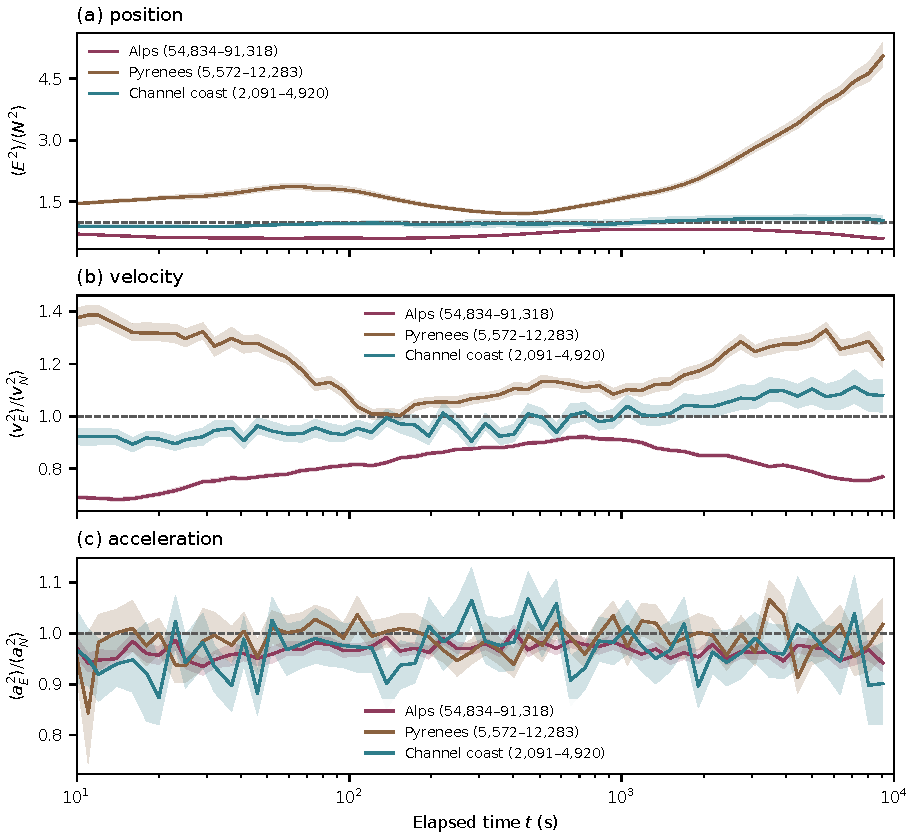
\includegraphics[width=\linewidth]{generated/kinematic_isotropy_terrain}
  \caption{Paraglider east/north second-moment ratios
by take-off region, against time since launch. Position, velocity and acceleration
all retain mean motion. Shading gives pointwise 10--90\% site--day bootstrap ranges;
times require \StatKinMinFlights\ flights and \StatKinMinClusters\ clusters, with
flight-count ranges in the legends. Missing site/date records form singleton groups.
Unity marks equal component moments, leaving cross moments and angular structure
untested. Panel limits follow each quantity; no scaling exponent is fitted.}
  \label{fig:kinematic-isotropy-terrain}
  \label{fig:kinematic-isotropy}
\end{figure}

\begin{figure}[p]
 \centering
 \IfFileExists{generated/kinematic_isotropy_terrain_level.pdf}{%
 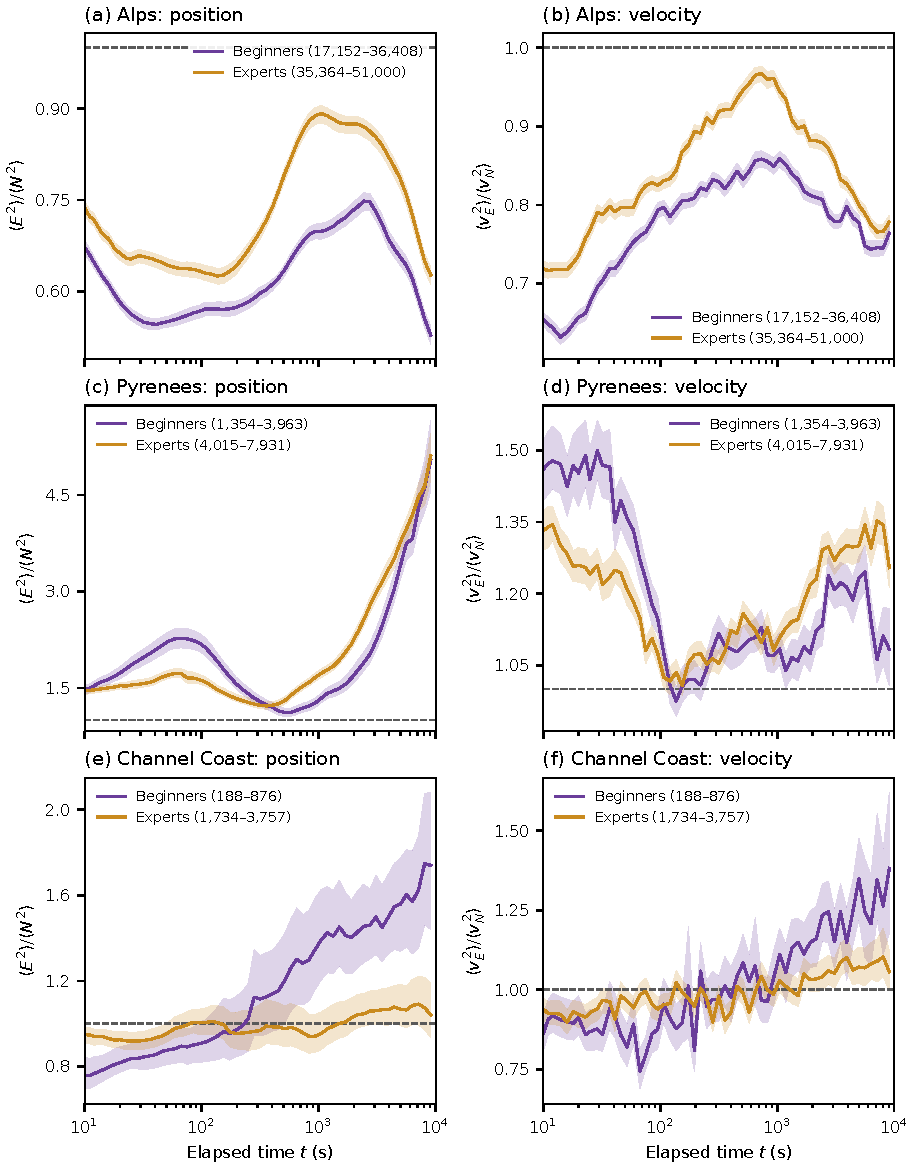
\includegraphics[width=\linewidth]{generated/kinematic_isotropy_terrain_level}%
 }{\fbox{\parbox{.8\linewidth}{Equipment comparisons await the complete rebuild.}}}
 \caption{Paraglider second-moment ratios within each
take-off region: beginners (EN A/B, violet) and experts (EN C/D/CCC, ochre), using
equipment as an experience proxy. Tandem, non-certified and unclassified records
are excluded. Pointwise bootstrap bands and support minima follow
Fig.~\ref{fig:kinematic-isotropy-terrain}.}
 \label{fig:kinematic-equipment}
\end{figure}

\FloatBarrier
\paragraph{Equipment within each region.}
EN A/B and EN C/D/CCC provide the beginners and experts proxies of
Sec.~\ref{sec:glider}. In the Alps, the C/D/CCC position and velocity ratios
remain closer to unity at all displayed supported times. The median position
ratio is \StatKinTerrainAlpsEquipmentCDCCCPositionMedian, versus
\StatKinTerrainAlpsEquipmentABPositionMedian\ for A/B. The Pyrenees and coastal
contrasts do not have the same ordering across all times and quantities.

\begin{figure}[p]
 \centering
 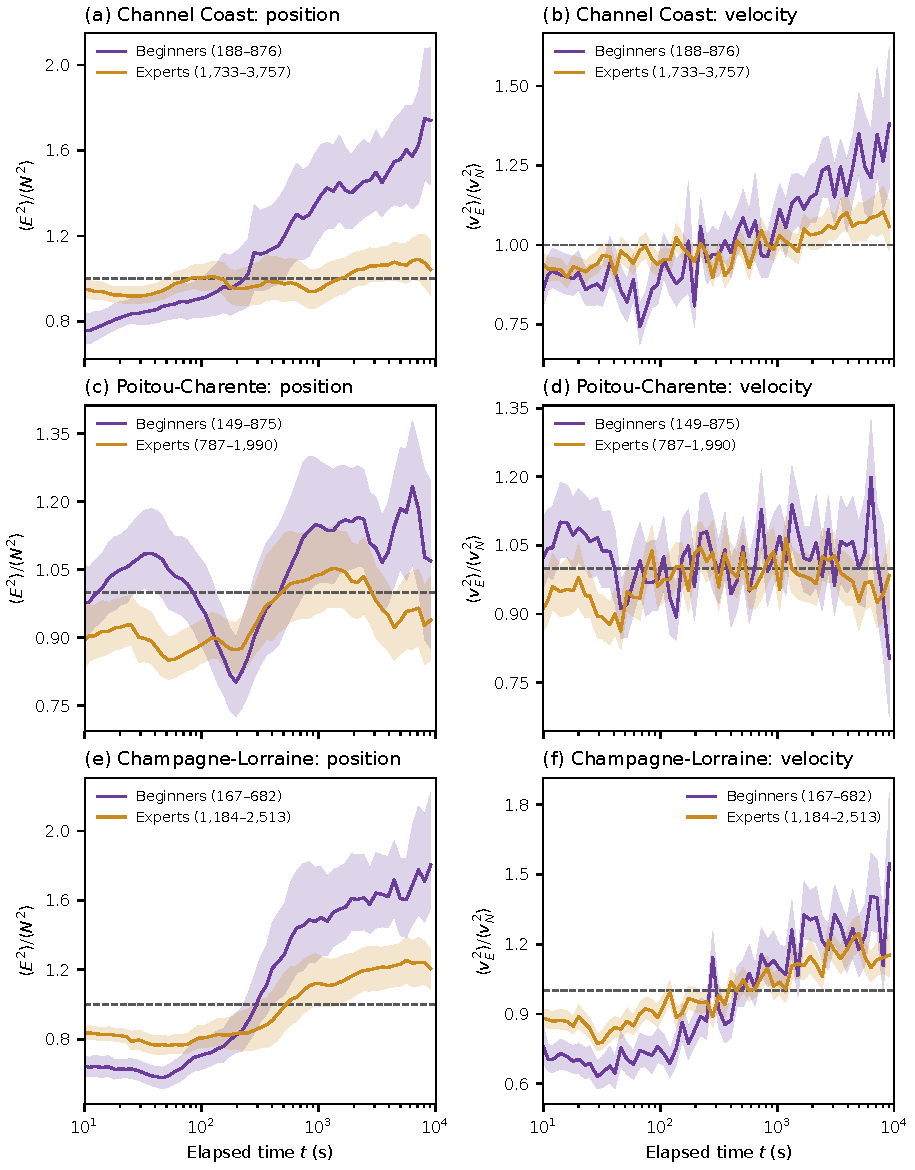
\includegraphics[width=\linewidth]{generated/kinematic_isotropy_flat_level}
 \caption{Equipment contrasts in three take-off boxes outside the mountain
 comparison: Channel Coast, Poitou-Charente and Champagne-Lorraine. Position and
 velocity ratios use the paired support, pointwise 10--90\% site--day bootstrap
 bands and display minima of Fig.~\ref{fig:kinematic-equipment}. The coastal row
 is repeated to compare it directly with the two additional regions. The boxes
 label take-off locations; they do not measure terrain exposure along each route
 or match wind conditions between equipment groups.}
 \label{fig:kinematic-low-relief}
\end{figure}


\paragraph{An interpretation to test.}
The smaller east--north imbalance of the C/D/CCC group in the Alps and over much
of the coastal comparison motivates a hypothesis: equipment and pilot decisions
may moderate the directional constraints associated with wind and terrain. A wing
with different flight characteristics may permit different routes, while a pilot's
choices may alter how a route follows the local lift and wind. Similar mountain
profiles could reflect a shared geographical constraint, with a difference in its
magnitude between groups. This is a possible explanation of the observed contrasts,
rather than a measured decomposition of their causes.

The Pyrenean curves limit that explanation. Their ordering reverses with elapsed
time, and the C/D/CCC group does not remain uniformly closer to one in either
position or velocity. Near \SI{9086}{\second}, the position ratios are about
\num{5.05} for A/B and \num{5.11} for C/D/CCC. The coastal position contrast is
larger at the same time, about \num{1.74} versus \num{1.04}, but its support is
also unequal: \num{188} versus \num{1733} paired flights. The bands are pointwise
10--90\% site--day bootstrap ranges, not simultaneous confidence bands or a direct
confidence interval for a between-group difference.

\paragraph{What proximity to unity establishes.}
The ratio compares two ensemble raw second moments. It does not measure the
isotropy of each flight or the ability of an individual pilot to make progress
against wind. For example, a centred Gaussian with covariance
\[
 \begin{pmatrix}1&0.9\\0.9&1\end{pmatrix}
\]
has equal east and north second moments but a principal-variance ratio of 19.
For a general centred law, a covariance proportional to the identity establishes
only a second-order condition, rather than rotational invariance of the full
distribution. A mixture
of strongly east-directed and strongly north-directed routes can also balance
ensemble moments while each route remains directional. Deliberately following a
downwind cross-country route may be successful flight despite that directionality.

\paragraph{Equipment, terrain and selection.}
EN A/B and EN C/D/CCC are equipment groups used as experience proxies. Actual pilot
skill is unmeasured, and an experienced pilot can fly an A/B wing. Certification
classes describe tested flight behaviour and associated pilot requirements; the
class is not itself a measured aerodynamic performance ranking
\cite{dhv_classification}. Equipment, pilot selection and intended task therefore
remain entangled in these comparisons.

The Channel Coast box is also not a wind-only experiment. It includes coastal
cliffs and valleys, including those documented in the Pays de Caux
\cite{dreal_pays_de_caux}. Wind and terrain may jointly orient lift and routes.
Moreover, the boxes classify take-off locations rather than terrain exposure along
the entire flight. The additional Poitou-Charente and Champagne-Lorraine comparisons
in Fig.~\ref{fig:kinematic-low-relief} extend the geographical description, but these
broad boxes are not verified terrain polygons or meteorologically matched controls.
The Poitou-Charente curves cross with broad overlapping bands; the later
Champagne-Lorraine position contrast also leaves the C/D/CCC ratio above one.
Thus the coastal pattern does not establish a general flatland mechanism.

\paragraph{Discriminating comparisons.}
A first comparison would restrict both equipment groups to overlapping take-off
sites and days, with comparable duration and task. This would test whether the
contrast survives closer matching of observed conditions; the current cluster
bootstrap adjusts the uncertainty for one grouping structure without performing
that matching. Mean ground drift, centred directional variability and the mixture
of individual route directions should then be distinguished. The independent
regional references in Sections~\ref{sec:independent-terrain-axis}
and~\ref{sec:independent-coastal-wind} provide an initial alignment comparison;
wind matched to flight times and local terrain along tracks would test the
proposed mechanisms more directly.
Where records permit it, comparisons of the same pilot using different wings could
help assess equipment and pilot selection separately. Before describing any of
these contrasts as resistance to wind, the target needs to be defined: upwind
progress, air-relative performance and the choice of route are different outcomes.

\paragraph{Wind and ground velocity.}

The kinematic relation
\begin{equation}
  \mathbf v_{\mathrm{ground}}=\mathbf v_{\mathrm{air}}+\mathbf w_h
  \label{eq:ground-air-wind}
\end{equation}
prevents ground velocity alone from separating still-air motion and wind.
Route choice and net progress also enter the mean. Differentiation removes a
constant wind contribution but retains changing wind and manoeuvres.

If the wind field is $\mathbf w_h(\mathbf r,z,t)$, its derivative along the trajectory is
\begin{equation}
 \mathbf a_{\mathrm{ground}}
 =\frac{\mathrm d\mathbf v_{\mathrm{air}}}{\mathrm dt}
  +\partial_t\mathbf w_h
  +(\mathbf v_{\mathrm{ground}}\!\cdot\nabla_h)\mathbf w_h
  +\dot z\,\partial_z\mathbf w_h.
 \label{eq:wind-acceleration}
\end{equation}
Thus even a time-independent wind field contributes to acceleration when the glider
crosses spatial gradients.

Separating these effects requires terrain alignment and independent wind estimates
within matched region and site--day groups. Thermal-centre drift may help after
segmentation, subject to assumptions about thermal motion. Randomly rotating flights
offers an alignment control: it balances pooled directions while preserving every
radial displacement, without reconstructing still-air motion.

\FloatBarrier
\subsection{Regional changes of velocity and direction}
\label{sec:regional-variations}

Second differences permit a regional comparison that is insensitive to an added
constant velocity. Their physical scale can be expressed without fitting an exponent.
For the two adjacent interval-mean ground velocities,
\begin{equation}
 \overline{\mathbf v}_1=\frac{\mathbf r(t+\tau)-\mathbf r(t)}{\tau},\qquad
 \overline{\mathbf v}_2=\frac{\mathbf r(t+2\tau)-\mathbf r(t+\tau)}{\tau},\qquad
 D_2(\tau)=\frac{\sqrt{V_2(\tau)}}{\tau}
 =\sqrt{\mathbb E|\overline{\mathbf v}_2-\overline{\mathbf v}_1|^2}.
 \label{eq:variation-velocity-change}
\end{equation}
Thus $D_2$, in \si{\metre\per\second}, measures changes of the mean velocity vector
between adjacent intervals. Both changes of direction and changes of its magnitude
contribute. This identity requires neither stationary increments nor self-similarity.
It does not measure wind speed.

The focused measurement uses all \num{\StatVarParaRegionalFlights} paraglider and
\num{\StatVarHangRegionalFlights} hang-glider flights in the three regional take-off
boxes. It reads the verified common-grid coordinates used by the regional PCA,
without repeating cleaning or limiting the number of flights. Eighteen physical
lags span \SIrange{10}{10000}{\second}; the four display lags agree with the updated
PCA at 10, 100, 1000 and \SI{10000}{\second}. Segment boundaries remain mandatory.

Three support conventions answer different questions. The available-origin curves
use every supported origin for each order separately, spaced by $\tau$ within each
segment. The matched-order comparison uses the same origins and flights for orders
one, two and three, and therefore requires $3\tau$ of continuous support. These
stencils overlap even though consecutive origins are separated by $\tau$. A further
common-origin control uses every 10-s origin supporting a continuous 3000-s window,
and retains that exact set for every order and every lag through \SI{1000}{\second}.
The 1000-s limit is a declared support convention; it avoids selecting only flights
with 30,000-s continuous records merely to compare the smaller scales.

Within each flight, eligible origins are pooled before flights receive equal weight.
The report also retains the pooled-origin result used as a weighting sensitivity.
This distinguishes the estimator here from the pooled-origin PCA in
Sec.~\ref{sec:transport-anisotropy}. Uncertainty uses 500 bootstrap draws of complete
site--day groups, jointly across lags and difference orders. Missing group keys
occur in three Alpine paraglider flights and are treated as singleton groups.
Pointwise 95\% intervals require at least 20 contributing groups and 90\% finite
replicates; this display threshold is not a guarantee of coverage. Regional
RMS-change ratios additionally receive approximate simultaneous 95\% bands over
their supported lag grid, obtained from the bootstrap maximum standardised
log-ratio deviation. The interpretation assumes independently resampleable groups;
dependence across sites, dates or repeated pilots can remain.

\begin{figure}[htbp]
 \centering
 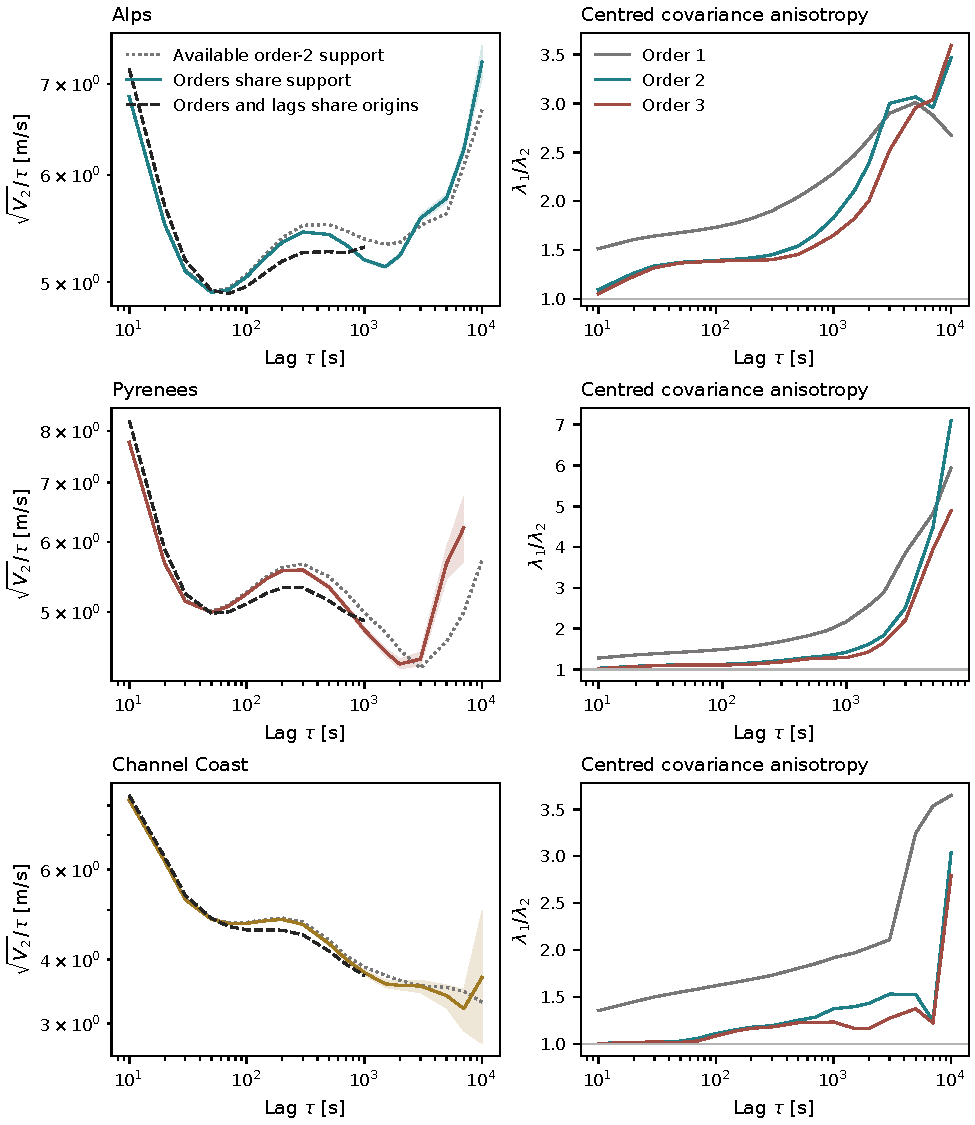
\includegraphics[width=.94\linewidth]{generated/ch3_regional_variations}
 \caption{Regional changes of ground velocity in paragliders. Left: $D_2$ on
 available order-two support, on support shared by orders one to three, and on
 origins common to all orders and lags through 1000~s. Shading is the pointwise
 site--day interval for the matched-order curve. Right: covariance eigenvalue
 ratios on the same matched origins. Curves are omitted where fewer than eight
 flights contribute; all numerical cells remain in the report. Support at the
 long end is shown in Fig.~\ref{fig:variation-support}.}
 \label{fig:regional-variations}
\end{figure}

For directionality, retain the vector $\mathbf d_2=A_2\mathbf r$ before taking its
squared norm. Its mean and centred covariance satisfy
\begin{equation}
 \boldsymbol\mu_2=\mathbb E\mathbf d_2,\qquad
 C_2=\operatorname{Cov}(\mathbf d_2),\qquad
 V_2=\operatorname{tr}C_2+|\boldsymbol\mu_2|^2.
 \label{eq:variation-covariance}
\end{equation}
The covariance includes variation between flight means as well as within flights.
The ratio of its eigenvalues measures directional imbalance of the dispersion;
the scalar $V_2$ alone cannot do so. As before, the leading axis has no signed
direction and becomes poorly determined near equal eigenvalues.

\begin{table}[htbp]
 \centering\small
 \caption{Paraglider diagnostics at \SI{\StatVarReferenceLagS}{\second}, with
 equal flight weights and origins shared by all three difference orders.
 The eigenvalue ratios refer to centred covariances at the indicated order.}
 \label{tab:regional-variations}
 \begin{tabular}{@{}lrrrrr@{}}\toprule
 Region & Flights & $D_2$ [m/s] & Ratio, order 1 & Ratio, order 2 & $V_3/V_2$\\\midrule
 Alps & \num{\StatVarParaAlpsFlights} & \StatVarParaAlpsRmsMatched & \StatVarParaAlpsRatioOne & \StatVarParaAlpsRatioTwo & \StatVarParaAlpsOrderRatio\\
 Pyrenees & \num{\StatVarParaPyreneesFlights} & \StatVarParaPyreneesRmsMatched & \StatVarParaPyreneesRatioOne & \StatVarParaPyreneesRatioTwo & \StatVarParaPyreneesOrderRatio\\
 Channel Coast & \num{\StatVarParaCoastFlights} & \StatVarParaCoastRmsMatched & \StatVarParaCoastRatioOne & \StatVarParaCoastRatioTwo & \StatVarParaCoastOrderRatio\\\bottomrule
 \end{tabular}
\end{table}

At this lag, second differencing reduces the covariance anisotropy relative to
ordinary increments in all three regions, but leaves a directional contrast
(Table~\ref{tab:regional-variations}). The order-two axes are about
\SI{\StatVarParaAlpsAngleTwo}{\degree},
\SI{\StatVarParaPyreneesAngleTwo}{\degree} and
\SI{\StatVarParaCoastAngleTwo}{\degree} counterclockwise from east.
At 10~s the second-difference covariance is much closer to equal principal
variances, especially on the coast; an angle there should not be interpreted as
a resolved environmental orientation.

\begin{figure}[htbp]
 \centering
 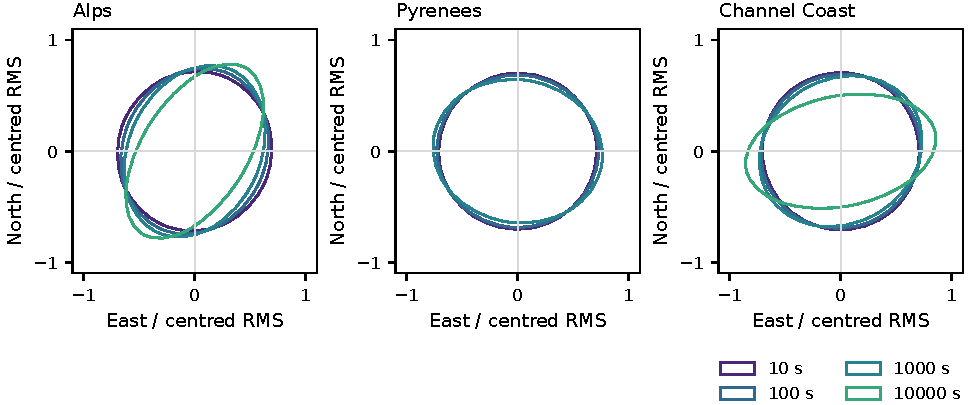
\includegraphics[width=\linewidth]{generated/ch3_variation_axes}
 \caption{Centred second-difference covariance ellipses, normalised by their own
 trace, on matched-order origins. Colours use the same four physical lags as the
 regional PCA. Normalisation removes amplitude and the ellipses omit the mean.
 The Pyrenean 10,000-s ellipse is not shown because only three flights contribute.}
 \label{fig:variation-axes}
\end{figure}

Holding origins fixed through 1000~s gives $D_2$ values of
\SI{\StatVarParaAlpsRmsCommon}{\metre\per\second} in the Alps,
\SI{\StatVarParaPyreneesRmsCommon}{\metre\per\second} in the Pyrenees and
\SI{\StatVarParaCoastRmsCommon}{\metre\per\second} on the coast at 1000~s.
The Alpine-to-coastal ratio is \num{\StatVarParaAlpsVsCoastRatio}, with simultaneous
band \num{\StatVarParaAlpsVsCoastLower}--\num{\StatVarParaAlpsVsCoastUpper}; the
Alpine-to-Pyrenean ratio is \num{\StatVarParaAlpsVsPyreneesRatio}, with band
\num{\StatVarParaAlpsVsPyreneesLower}--\num{\StatVarParaAlpsVsPyreneesUpper}.
The ordering changes with lag: at 10~s the coastal and Pyrenean values exceed the
Alpine value. Similar-looking mountain curves therefore do not establish regional
equality, and a single regional amplitude ratio does not describe the whole interval.

A descriptive standardisation further restricts the common-origin population to
shared strata of declared open/closed task, retained duration (up to 2~h, 2--4~h,
over 4~h), season period (through 2009, 2010--2019, 2020 onward) and equipment
(EN A/B or EN C/D/CCC). Each retained stratum needs at least ten flights per
region; its target mass is proportional to its smallest regional count.
Unknown context labels are excluded from this control. The resulting
\num{\StatVarParaStandardStrata} strata retain
\num{\StatVarParaAlpsStandardFlights}, \num{\StatVarParaPyreneesStandardFlights} and
\num{\StatVarParaCoastStandardFlights} flights. Their standardised 1000-s values
are respectively \SI{\StatVarParaAlpsRmsStandard}{\metre\per\second},
\SI{\StatVarParaPyreneesRmsStandard}{\metre\per\second} and
\SI{\StatVarParaCoastRmsStandard}{\metre\per\second}. The coastal contrast remains
in these point estimates; calibrated intervals for the standardised contrasts are
not supplied. No three-region common equipment/context strata survive for hang gliders.

\begin{figure}[htbp]
 \centering
 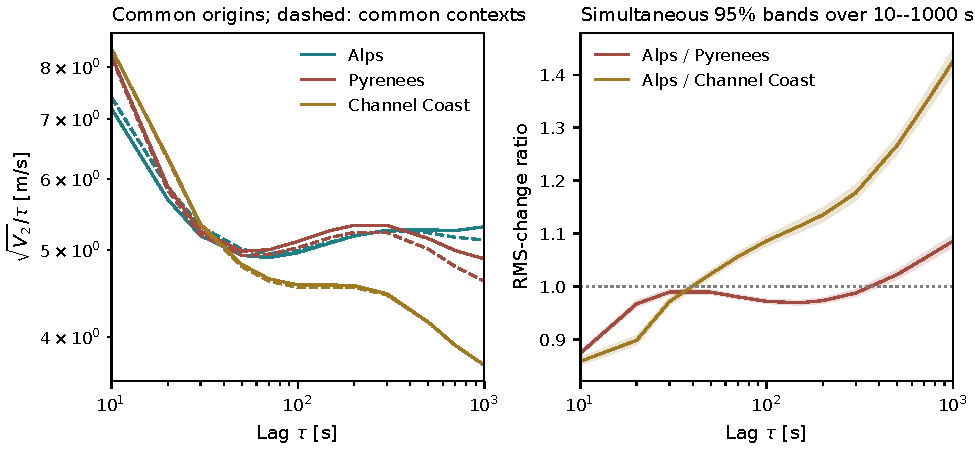
\includegraphics[width=\linewidth]{generated/ch3_variation_controls}
 \caption{Paraglider population controls. Left: common-origin curves, with the
 common-context standardisation dashed. The dashed curves are descriptive point
 estimates. Right: regional ratios of the unstandardised common-origin curves;
 shading is simultaneous over the 18-lag grid's supported subset through 1000~s.
 These controls do not match meteorology, local terrain exposure or pilot identity.}
 \label{fig:variation-controls}
\end{figure}

These findings constrain a wind explanation without identifying wind. If populations
differed only by an added constant velocity and otherwise shared the same residual
dynamics, their second differences would agree. Their measured differences require
more than that particular explanation. Spatial or temporal wind variation, route
geometry, manoeuvres and population selection remain possible contributors. The
coast has smaller changes of interval-mean velocity at 1000~s, rather than a larger
signal that could simply be labelled stronger wind. An environmental attribution
requires independent wind information and terrain alignment, ideally within sites
under contrasting conditions.

\subsection{Third differences and the distribution of changes}
\label{sec:regional-third-differences}

The third difference extends the cancellation by one polynomial degree:
\begin{equation}
 A_3\mathbf r=\mathbf r(t+3\tau)-3\mathbf r(t+2\tau)
              +3\mathbf r(t+\tau)-\mathbf r(t),\qquad
 V_3=\mathbb E|A_3\mathbf r|^2.
 \label{eq:third-difference}
\end{equation}
For $\mathbf r(t)=\mathbf r_0+\mathbf v_0t+\tfrac12\mathbf a t^2$ with constant
vector acceleration, $V_2=|\mathbf a|^2\tau^4$ while $V_3=0$. A smooth curved
trajectory generally retains both signals: locally $A_3\mathbf r$ is proportional
to $\mathbf r^{(3)}\tau^3$. Constant-speed circular motion is therefore not
eliminated by taking order three.

Under the same centred stationary-increment second-moment law used in
Eq.~\eqref{eq:variation-hurst}, algebra gives
\begin{equation}
 V_3=K\bigl(15-6\,2^{2H}+3^{2H}\bigr)\tau^{2H},\qquad
 \frac{V_3}{V_2}=\frac{15-6\,2^{2H}+3^{2H}}{4-2^{2H}},\quad 0<H<1.
 \label{eq:third-difference-hurst}
\end{equation}
The power law must hold through $3\tau$. Thus the order ratio, in addition to the
two slopes, is a consistency condition on that model. It equals three for Brownian
motion plus an arbitrary constant velocity. Agreement between orders would not
constitute independent data or certify removal of every environmental trend.

\begin{figure}[htbp]
 \centering
 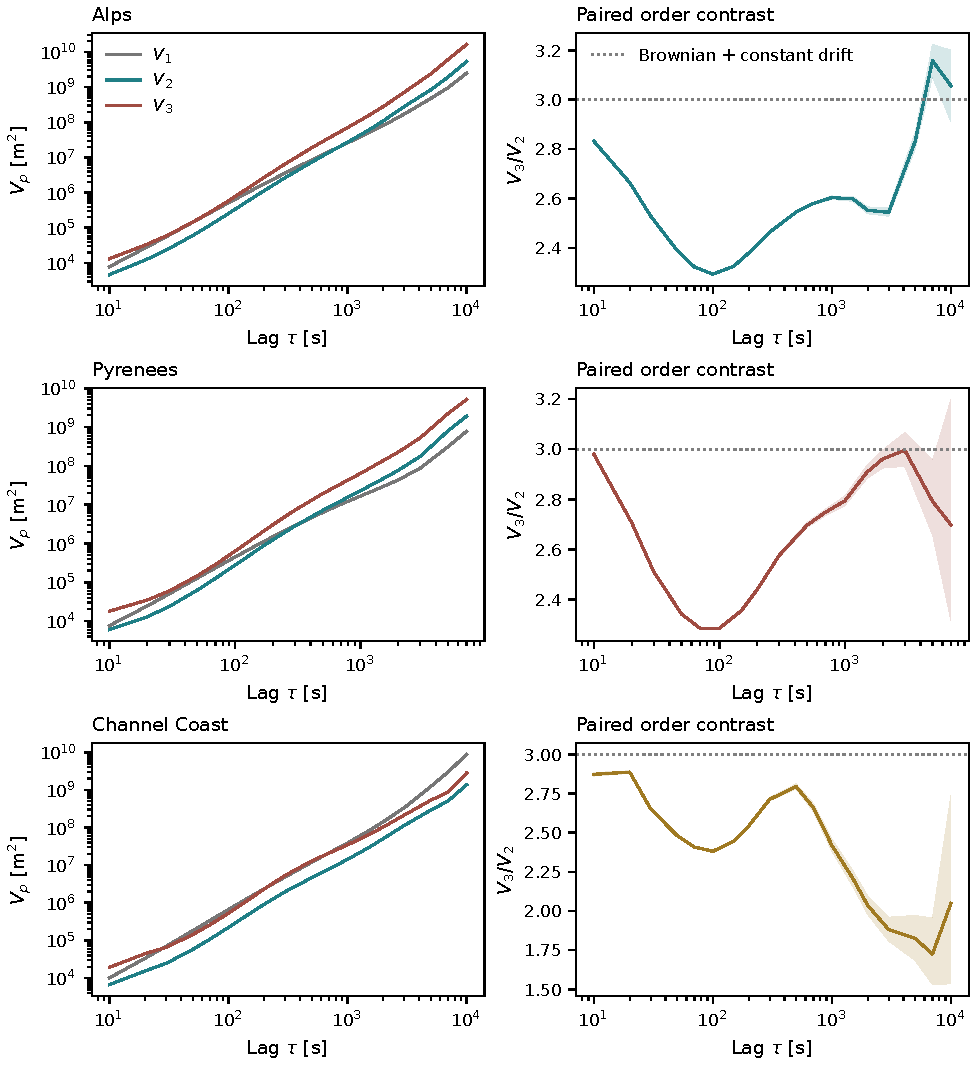
\includegraphics[width=.94\linewidth]{generated/ch3_variation_orders}
 \caption{Paraglider variations and their paired order ratio on identical origins.
 Different prefactors make the amplitudes of $V_2$ and $V_3$ directly unequal even
 under one scaling model. Right: $V_3/V_2$ with pointwise site--day intervals;
 the dotted line is the Brownian-plus-constant-velocity reference, not a fit.
 Fewer than eight contributing flights suppress a displayed curve cell.}
 \label{fig:variation-orders}
\end{figure}

The observed order ratios change with lag (Fig.~\ref{fig:variation-orders}).
At 100~s they are about 2.29 in both mountain regions and 2.38 on the coast;
at 1000~s they are \num{\StatVarParaAlpsOrderRatio},
\num{\StatVarParaPyreneesOrderRatio} and \num{\StatVarParaCoastOrderRatio}.
These curves supply a sensitivity and model-consistency diagnostic, without
establishing a scale-independent Hurst parameter. Order three also increases the
effect of independent position errors: variance $\sigma^2$ per coordinate adds
$6\sigma^2$ to the order-two scalar-component moment and $20\sigma^2$ to order
three. Correlated errors and smoothing alter those expressions. The 10-s end
therefore remains sensitive to acquisition and preprocessing resolution; a
calibrated sensor-noise subtraction is not performed here.

The distribution of $|A_2\mathbf r|/\tau$ supplies information lost by its second
moment. We retain equal-flight histogram probabilities and the squared-change
contribution of every bin, including zeros and both tails. Reported quantiles are
bin bounds, not interpolated exact sample quantiles. At 1000~s, the largest tenth
of changes accounts for approximately
\num{\StatVarParaAlpsTailShareLow}--\num{\StatVarParaAlpsTailShareHigh}\% of the
squared-change signal in the Alps,
\num{\StatVarParaPyreneesTailShareLow}--\num{\StatVarParaPyreneesTailShareHigh}\%
in the Pyrenees and
\num{\StatVarParaCoastTailShareLow}--\num{\StatVarParaCoastTailShareHigh}\% on the
coast. Each range reflects the unresolved boundary bin, not sampling uncertainty.
This measures concentration of the observable; it does not identify a flight
phase, turbulence or a tail-generating mechanism.

\begin{figure}[htbp]
 \centering
 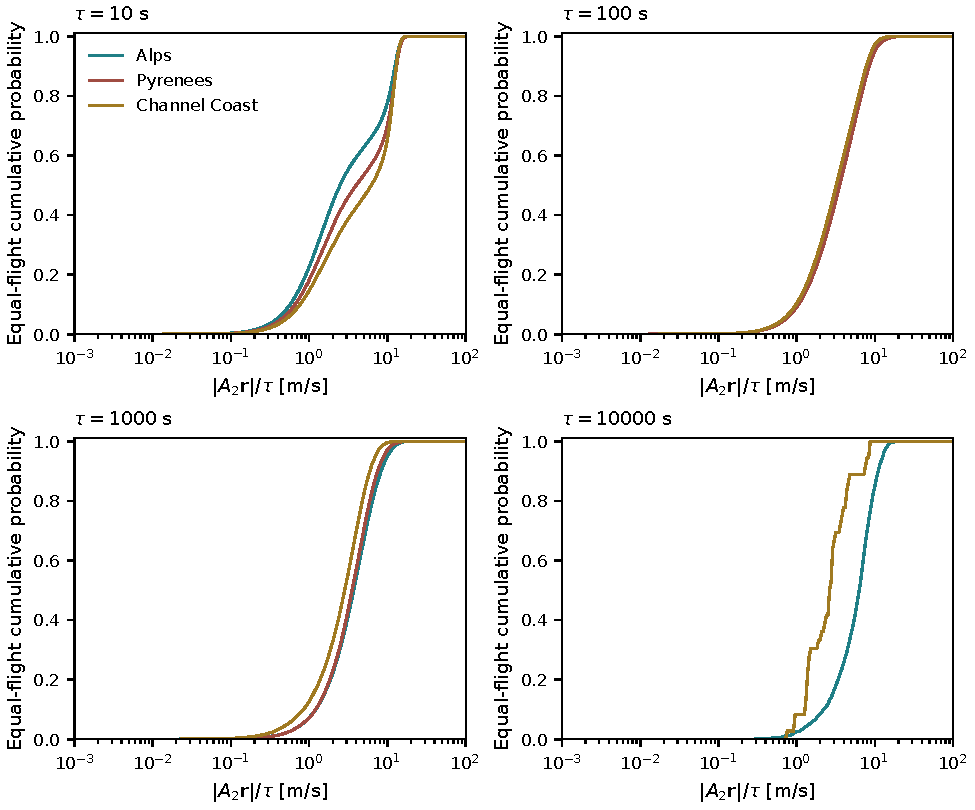
\includegraphics[width=\linewidth]{generated/ch3_variation_distributions}
 \caption{Equal-flight distributions of changes of interval-mean velocity at the
 four PCA display lags, using matched-order support. Curves are accumulated from
 fixed logarithmic bins; the complete report retains zero and overflow mass.
 No distribution is drawn for fewer than eight flights. The changing long-lag
 population must accompany comparisons between panels.}
 \label{fig:variation-distributions}
\end{figure}

\begin{figure}[htbp]
 \centering
 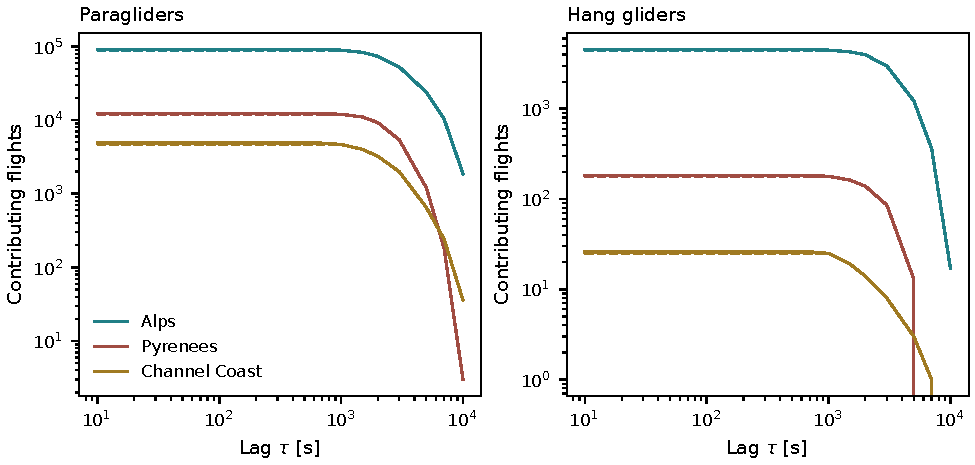
\includegraphics[width=\linewidth]{generated/ch3_variation_support}
 \caption{Contributing flights for matched orders (solid) and common origins
 through 1000~s (dashed). A matched observation requires $3\tau$ of continuous
 support. At 10,000~s the paraglider counts are
 \num{\StatVarParaAlpsMaxFlights}, \num{\StatVarParaPyreneesMaxFlights} and
 \num{\StatVarParaCoastMaxFlights}; hang-glider counts are
 \num{\StatVarHangAlpsMaxFlights}, \num{\StatVarHangPyreneesMaxFlights} and
 \num{\StatVarHangCoastMaxFlights}. All regional eligible flights enter where supported.}
 \label{fig:variation-support}
\end{figure}

